\documentclass[compress]{beamer}
\usepackage{ifthen,verbatim}

\title{Update on Track-Based Alignment in CRUZET}
\author{Jim Pivarski, Alexei Safonov, K\'aroly Banicz$^*$}
\institute{Texas A\&M University, $^*$US-CMS}
\date{23 July, 2008}

\newcommand{\isnote}{}
\xdefinecolor{lightyellow}{rgb}{1.,1.,0.25}
\xdefinecolor{darkblue}{rgb}{0.1,0.1,0.7}

%% Uncomment this to get annotations
%% \def\notes{\addtocounter{page}{-1}
%%            \renewcommand{\isnote}{*}
%% 	   \beamertemplateshadingbackground{lightyellow}{white}
%%            \begin{frame}
%%            \frametitle{Notes for the previous page (page \insertpagenumber)}
%%            \itemize}
%% \def\endnotes{\enditemize
%% 	      \end{frame}
%%               \beamertemplateshadingbackground{white}{white}
%%               \renewcommand{\isnote}{}}

%% Uncomment this to not get annotations
\def\notes{\comment}
\def\endnotes{\endcomment}

\setbeamertemplate{navigation symbols}{}
\setbeamertemplate{headline}{\mbox{ } \hfill
\begin{minipage}{5.5 cm}
\vspace{-0.75 cm} \small
\end{minipage} \hfill
\begin{minipage}{4.5 cm}
\vspace{-0.75 cm} \small
\begin{flushright}
\ifthenelse{\equal{\insertpagenumber}{1}}{}{Jim Pivarski \hspace{0.2 cm} \insertpagenumber\isnote/\pageref{numpages}}
\end{flushright}
\end{minipage}\mbox{\hspace{0.2 cm}}\includegraphics[height=1 cm]{../cmslogo} \hspace{0.1 cm} \includegraphics[height=1 cm]{../tamulogo} \hspace{0.01 cm} \vspace{-1.05 cm}}

\begin{document}
\frame{\titlepage}

%% \begin{notes}
%% \item This is the annotated version of my talk.
%% \item If you want the version that I am presenting, download the one
%% labeled ``slides'' on Indico (or just ignore these yellow pages).
%% \item The annotated version is provided for extra detail and a written
%% record of comments that I intend to make orally.
%% \item Yellow notes refer to the content on the {\it previous} page.
%% \item All other slides are identical for the two versions.
%% \end{notes}

\begin{frame}
\frametitle{Outline}
\begin{itemize}\setlength{\itemsep}{0.75 cm}
\item Updates in CSC Overlap procedure in CRUZET
\item Baseline procedure using StandAloneMuons in CRUZET-2
\end{itemize}
%% \hspace{-0.83 cm} \textcolor{darkblue}{\Large Outline2}
\end{frame}

%% \section*{First section}
%% \begin{frame}
%% \begin{center}
%% \Huge \textcolor{blue}{First section}
%% \end{center}
%% \end{frame}


\begin{frame}
\frametitle{CSC Overlap procedure}
\small

We have the residuals, we can minimize them, but is it {\it aligned?}

\vfill
Plots of residuals on ME+4/1 chamber 16 from fit to chamber 15:
\begin{enumerate}
\item Any two segments in neighboring chambers
\item Exactly two segments, nearly collinear (linear fit has $\chi^2/\mbox{ndf}$ $<$ 10)
\item Applied alignment procedure
\end{enumerate}

\vfill
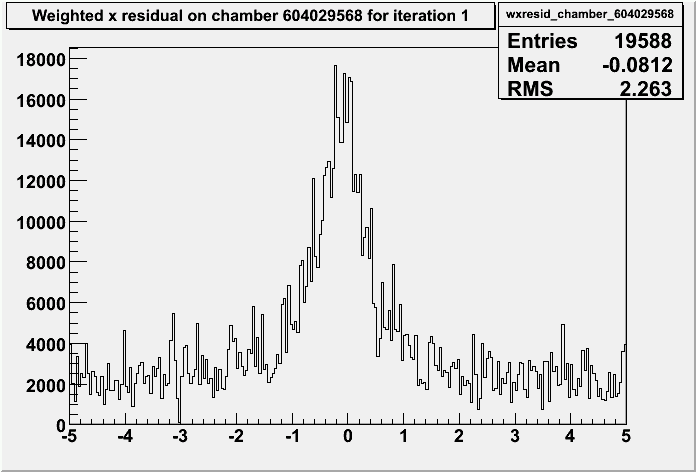
\includegraphics[height=3.5 cm]{before_cuts.png}
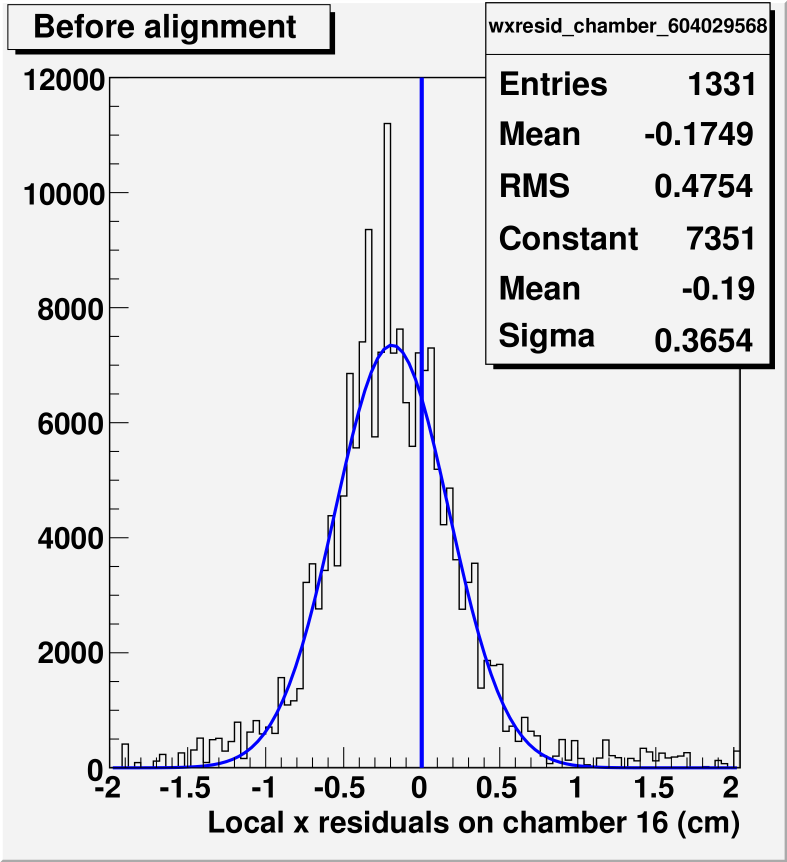
\includegraphics[height=3.5 cm]{before_alignment.png}
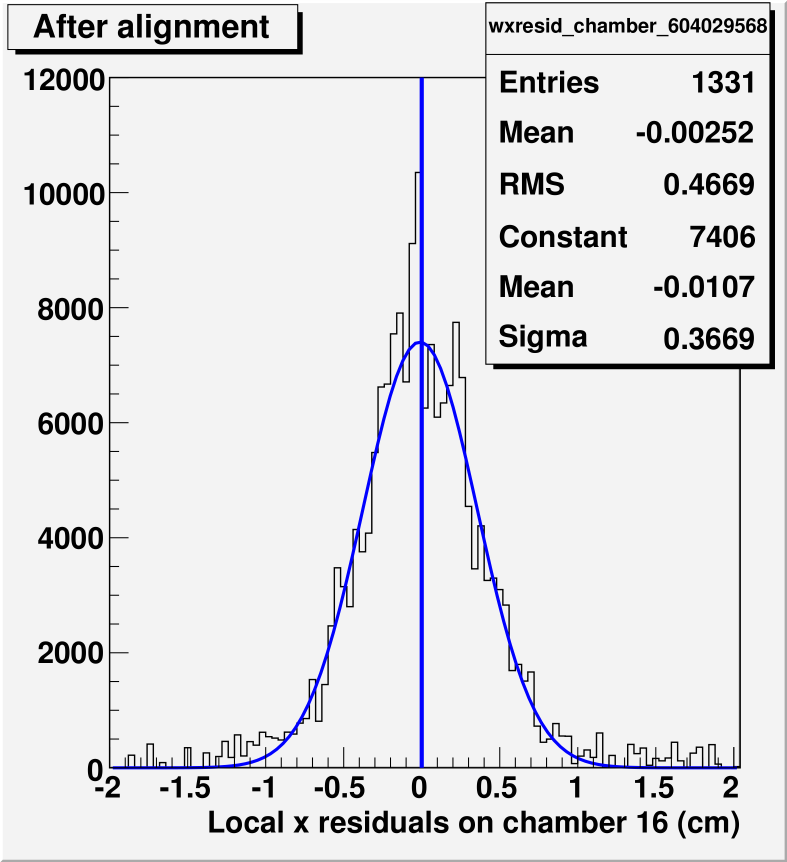
\includegraphics[height=3.5 cm]{after_alignment.png}

\end{frame}

\begin{frame}
\frametitle{Rings do not close}
\small

\begin{tabular}{p{0.5\linewidth} p{0.5\linewidth}}
ME+2/2 (CRUZET-1) & ME+3/2 (CRUZET-1) \\
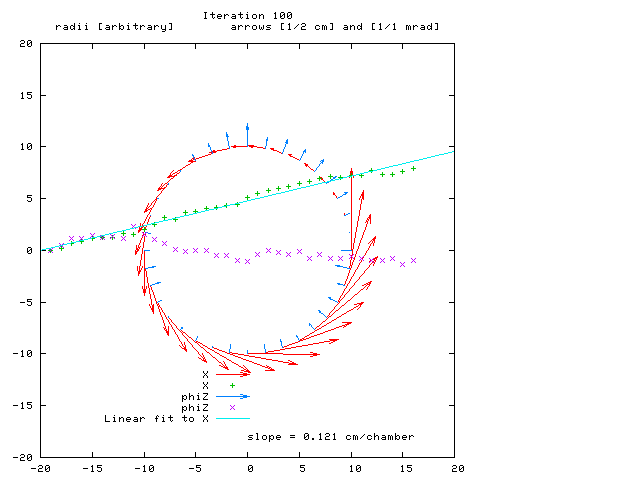
\includegraphics[width=\linewidth]{CRUZET1_MEplus22_plusIsRef_ch1fix_XphiZ.png} &
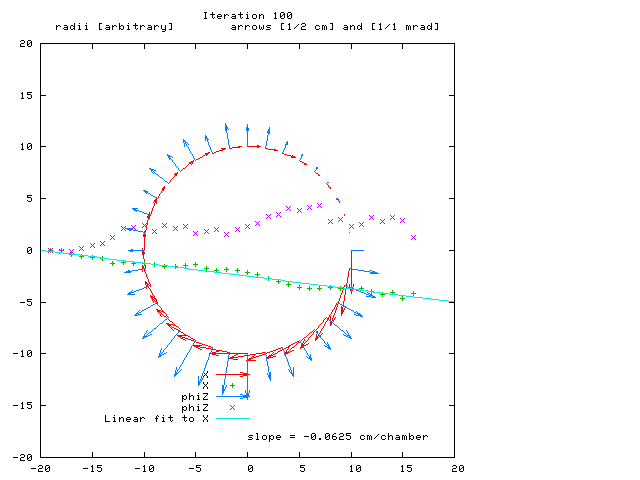
\includegraphics[width=\linewidth]{CRUZET1_MEplus32_plusIsRef_ch1fix_XphiZ.png}
\end{tabular}

\vspace{0.05 cm}
\begin{center}
Average alignment correction per chamber (confirmed in CRUZET-2)

\vspace{0.03 cm}
\renewcommand{\arraystretch}{1.2}
\begin{tabular}{c | c c c}
ring & ME+2 & ME+3 & ME+4 \\\hline
1 & $-0.5$~mm & ? & $+1.0$~mm \\
2 & $+1.2$~mm & $-0.6$~mm & \\
\end{tabular}
\end{center}

\vspace{0.05 cm} \scriptsize
{\it Iteration-by-iteration animations from CRUZET-1 and -2 available in}

\textcolor{blue}{\tt \underline{\href{https://banicz.web.cern.ch/banicz/CMS/alignment/CRUZET}{https://banicz.web.cern.ch/banicz/CMS/alignment/CRUZET}}}

\end{frame}

\begin{frame}
\frametitle{Interpretations}
\small

\vspace{0.5 cm}
\begin{columns}
\column{0.5\linewidth}
ME+2/2 with $R += 6.6$~mm

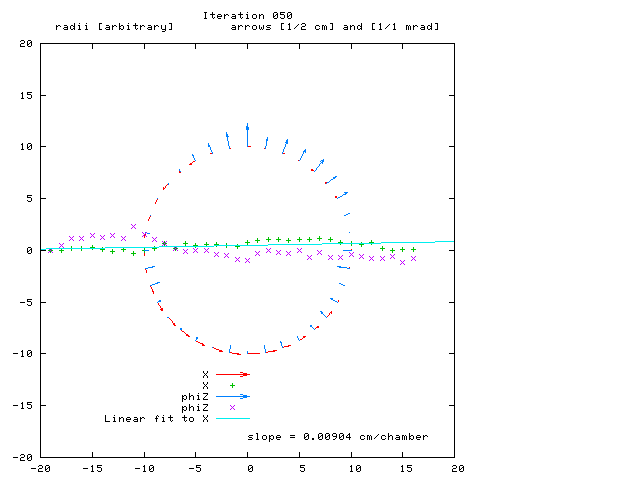
\includegraphics[width=\linewidth]{CRUZET1_MEplus22_Yf6_6mm_plusIsRef_ch1fix_XphiZ.png}

\column{0.5\linewidth}
Radial growth of the rings?

\renewcommand{\arraystretch}{1.2}
\begin{tabular}{c c}
ME+2/2 & ME+3/2 \\\hline
$+6.6$~mm & $-3$~mm
\end{tabular}

\begin{itemize}
\item ME2/2 and ME3/2 are identical: how can these be in opposite directions?
\item Hard to imagine a transcription error or a physical effect which can do this
\end{itemize}
\end{columns}

\vspace{0.5 cm}
However, Oleg and I have found that our narrow-end alignment pin positions in ideal DDD and ideal detector drawings do not agree.
\begin{itemize}
\item DDD is 7~mm too far from beamline in ME2/2 and ME3/2
\item 9.53~mm in all other stations (except ME1/1) very consistently
\item ME1/1 chambers have no alignment pins
\end{itemize}
\end{frame}

\begin{frame}
\frametitle{Wire group granularity?}

Discreteness of wire groups can cause an apparent radial shift

\begin{itemize}
\item for most hits, reconstructed $y$ is the nearest wire group center
\item at the edge of the chamber, $y$ is needed to resolve $x$
  position, propagating effect to $x$
\end{itemize}

\vfill
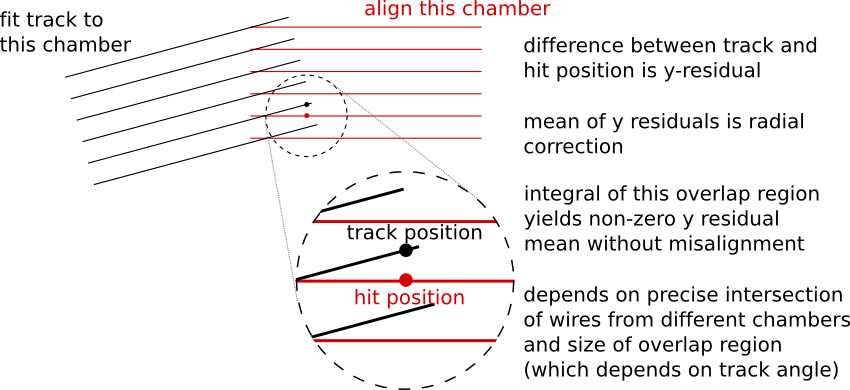
\includegraphics[width=\linewidth]{vertical_residual.png}

\end{frame}

\begin{frame}
\frametitle{Generating 6~mm shifts}
\small

\begin{itemize}
\item Beam-halo MC with ideal alignment
\item Overlay track extrapolated from reference (black) and hit (red)
\item Vertical difference between black and red is the $y$-residual
\item Can create a 6~mm $y$-residual by changing the degree of overlap
  (with cuts); cosmic rays have broader overlap due \mbox{to incidence angles\hspace{-1 cm}}
\end{itemize}

\mbox{ } \hfill 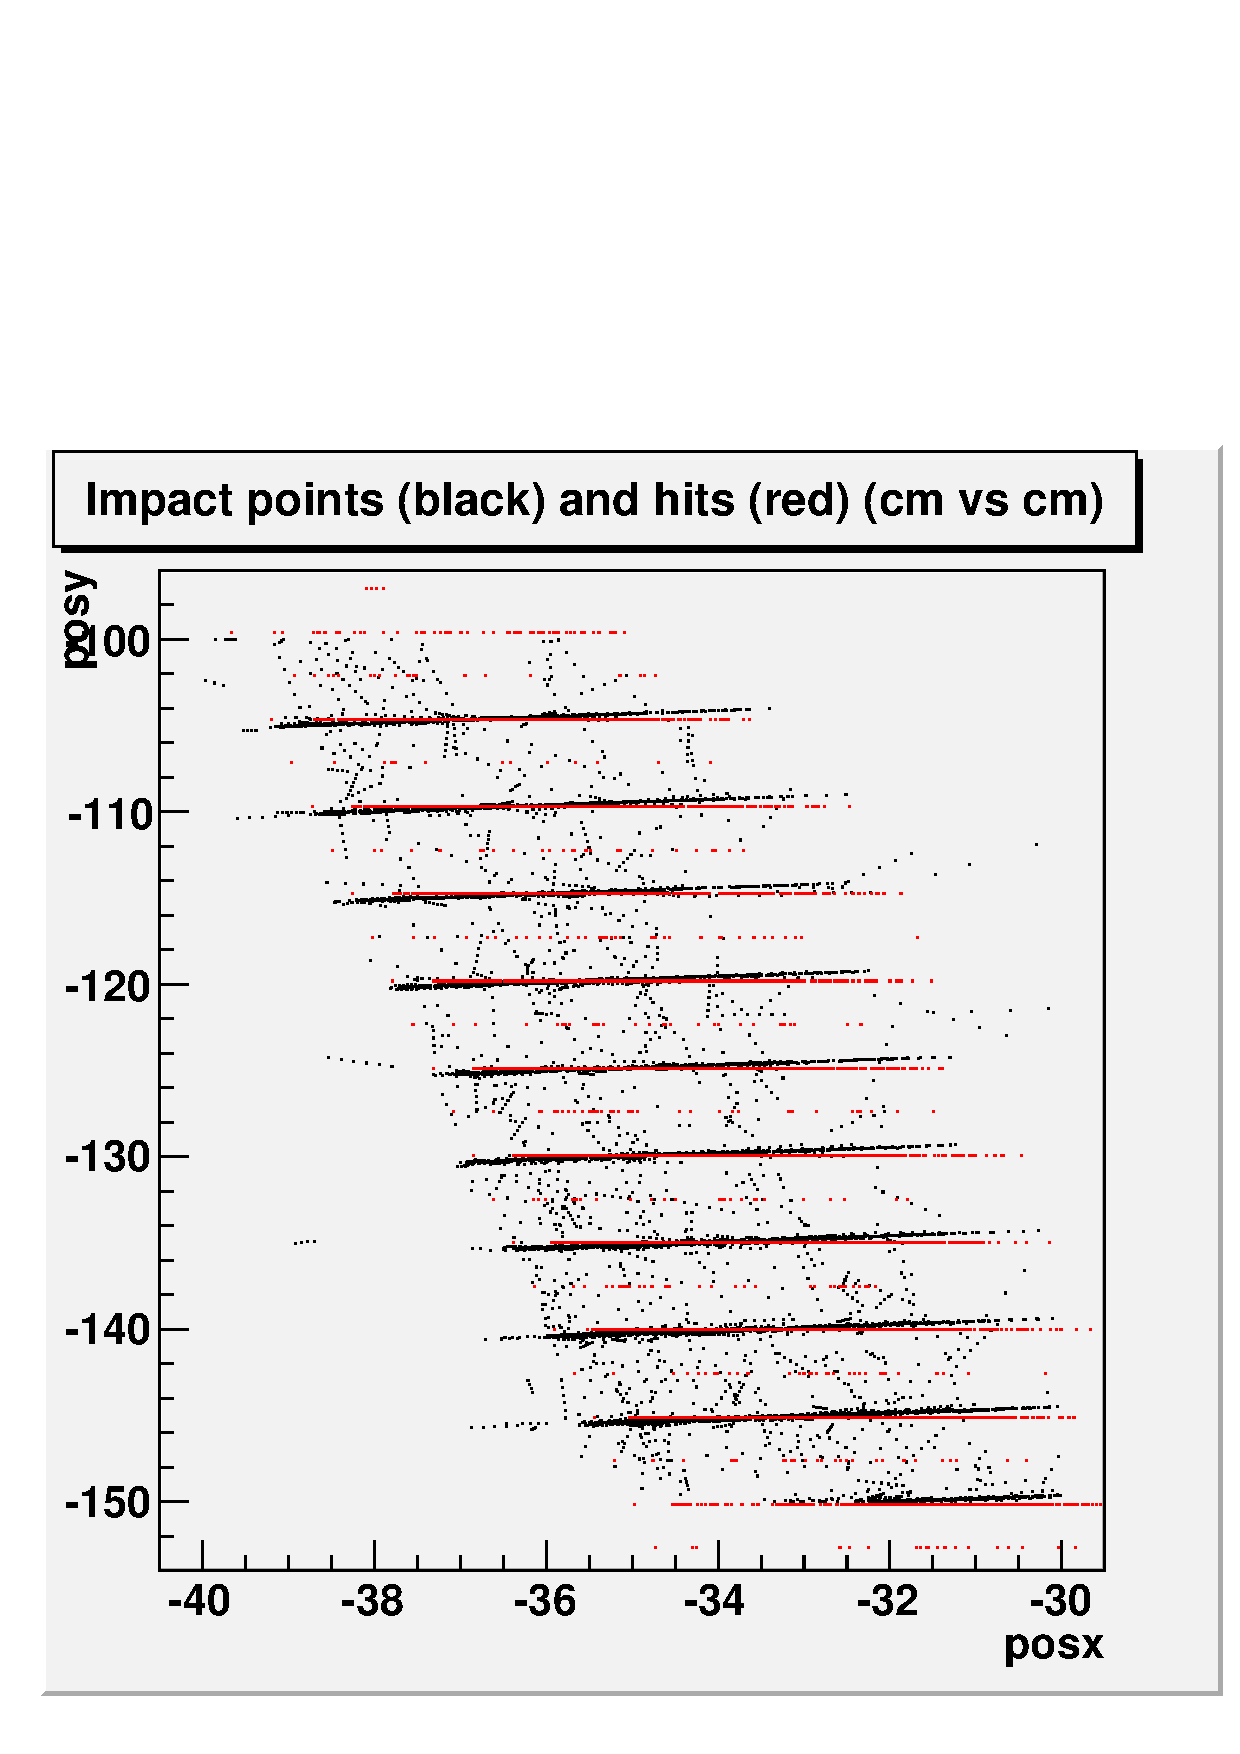
\includegraphics[width=0.45\linewidth]{selectioneffect_nocut.pdf}
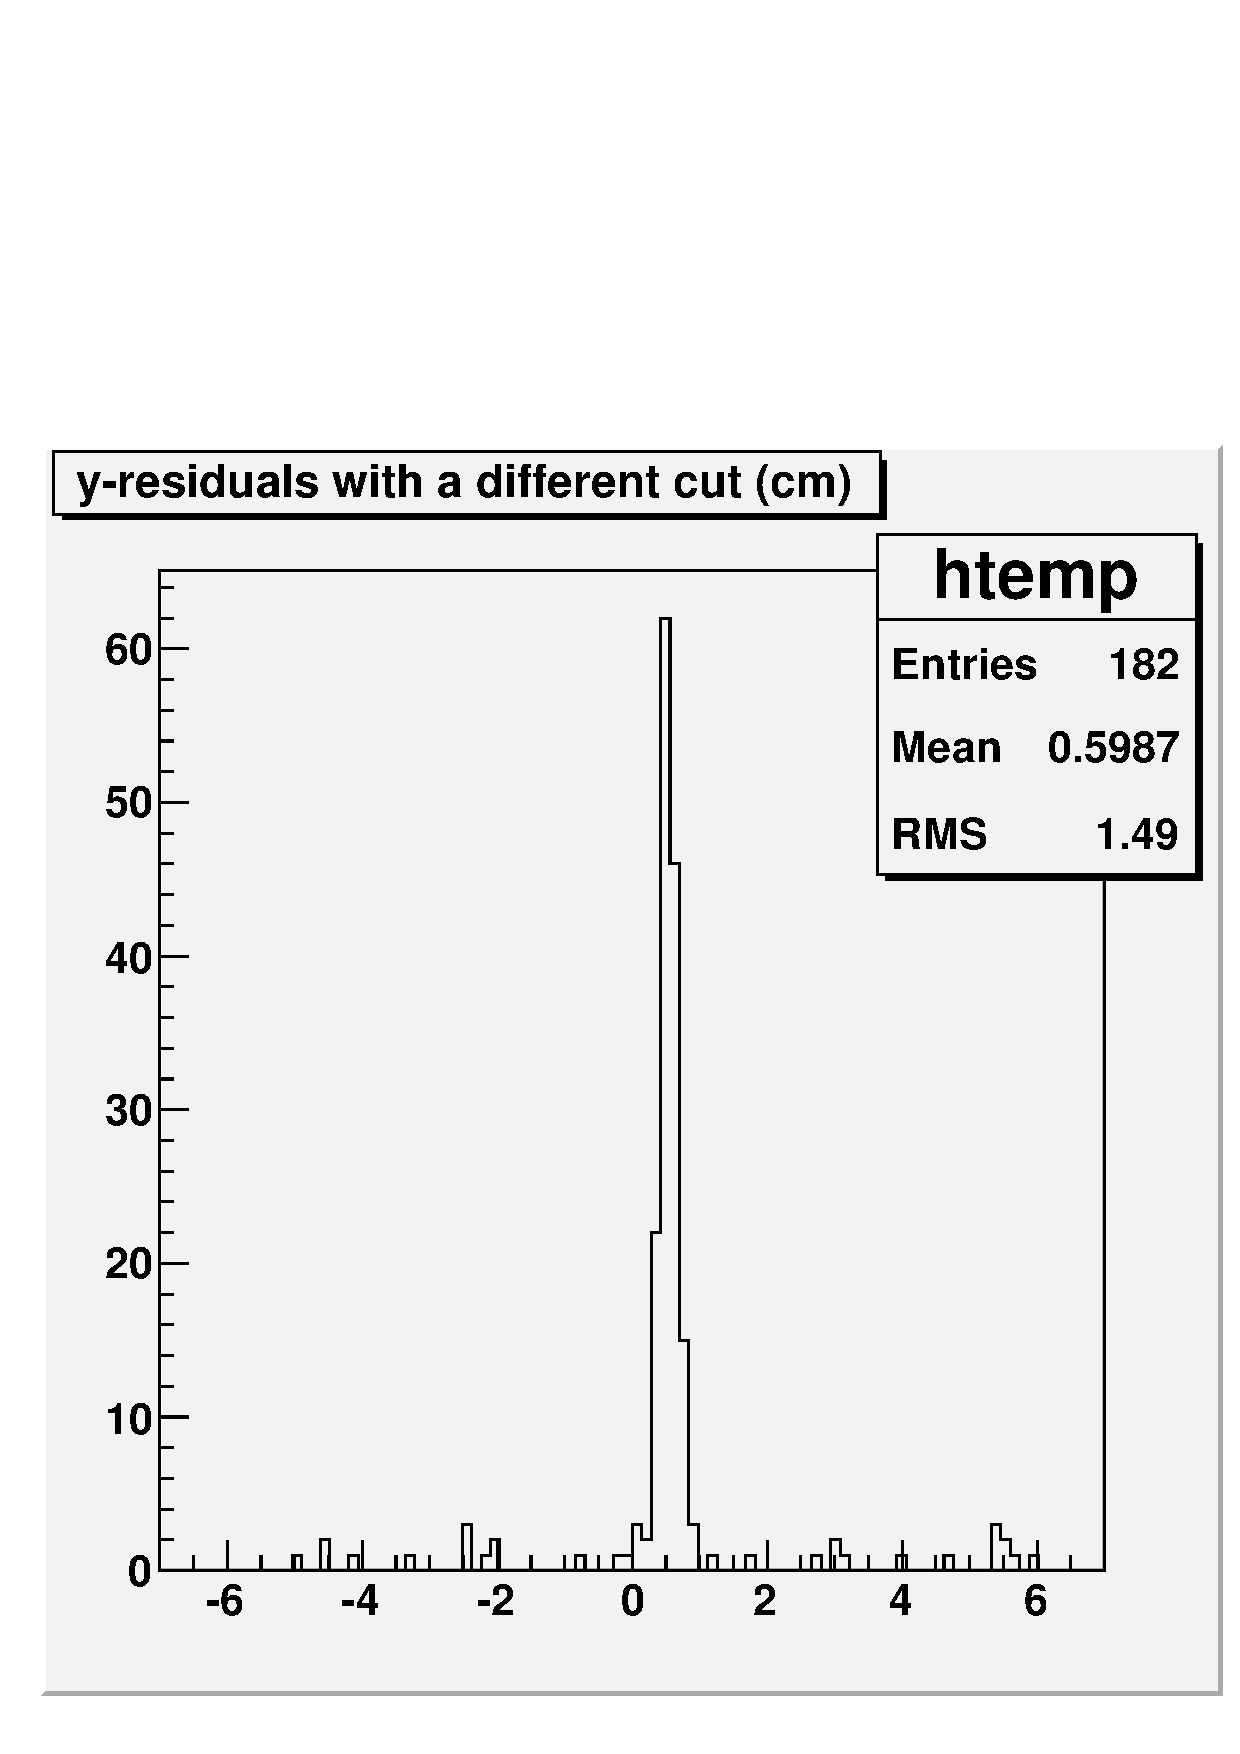
\includegraphics[width=0.45\linewidth]{selectioneffect_resid_withanothercut.pdf} \hfill \mbox{ }

\end{frame}

\begin{frame}
\frametitle{Baseline procedure in CRUZET}

Motivation: to look for the radial shift from further away, unaffected
by wire granularity (because you get to average over imperfections in
the reference tracking volume)

\vfill Method: fit tracks in muon barrel or one endcap station,
project them to another endcap station and align

\vfill Using HIP derivatives, we can get each hit to tell us where it
thinks the whole disk is (in $z$ for instance)

\vfill This is complimentary to Riccardo's geometric approach

\vfill Plots from CRUZET-2
\end{frame}

\begin{frame}
\frametitle{Finding the endcaps}

Fit tracks in the barrel, align endcap stations

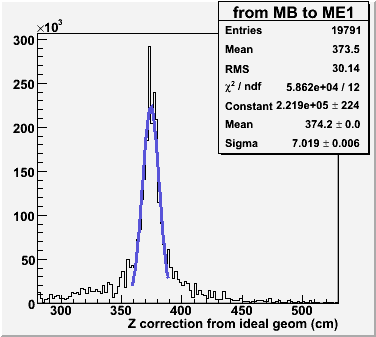
\includegraphics[width=0.4\linewidth]{hist_0and1.png}
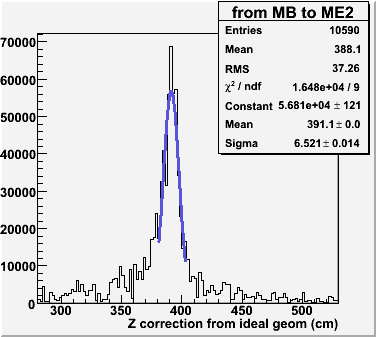
\includegraphics[width=0.4\linewidth]{hist_0and2.png}

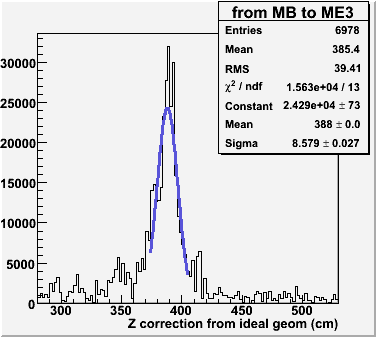
\includegraphics[width=0.4\linewidth]{hist_0and3.png}
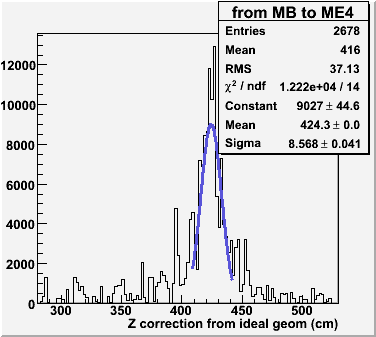
\includegraphics[width=0.4\linewidth]{hist_0and4.png}

\end{frame}

\begin{frame}
\frametitle{Finding the endcaps}

Fit tracks in ME1, align other endcap stations


\includegraphics[width=0.4\linewidth]{blank.png}
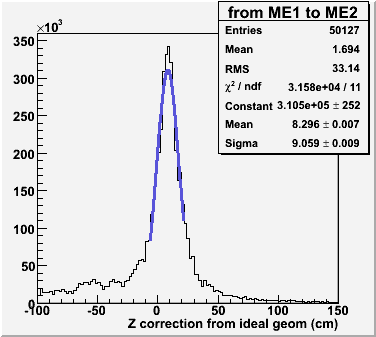
\includegraphics[width=0.4\linewidth]{hist_1and2.png}

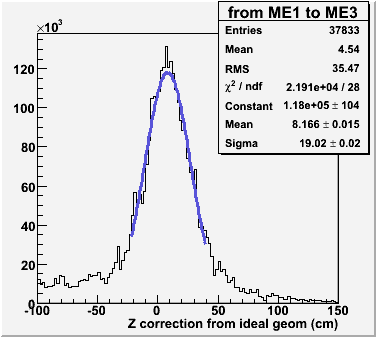
\includegraphics[width=0.4\linewidth]{hist_1and3.png}
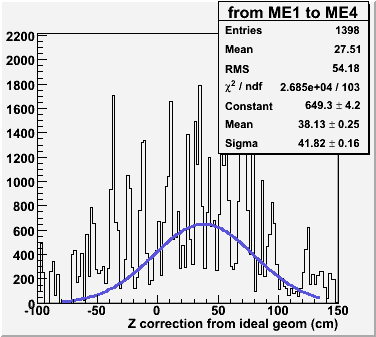
\includegraphics[width=0.4\linewidth]{hist_1and4.png}

\end{frame}

\begin{frame}
\frametitle{Finding the endcaps}

Fit tracks in ME2, align other endcap stations


\includegraphics[width=0.4\linewidth]{blank.png}

\includegraphics[width=0.4\linewidth]{blank.png}

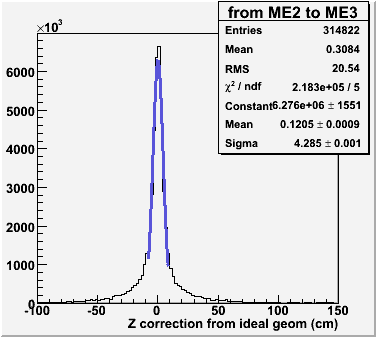
\includegraphics[width=0.4\linewidth]{hist_2and3.png}
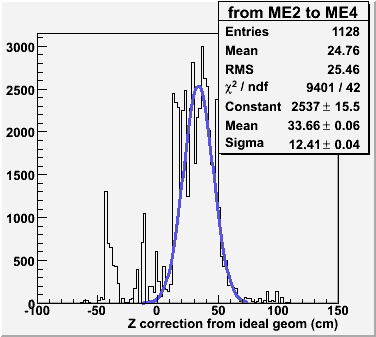
\includegraphics[width=0.4\linewidth]{hist_2and4.png}

\end{frame}

\begin{frame}
\frametitle{Finding the endcaps}

Fit tracks in ME3, align other endcap stations


\includegraphics[width=0.4\linewidth]{blank.png}

\includegraphics[width=0.4\linewidth]{blank.png}


\includegraphics[width=0.4\linewidth]{blank.png}
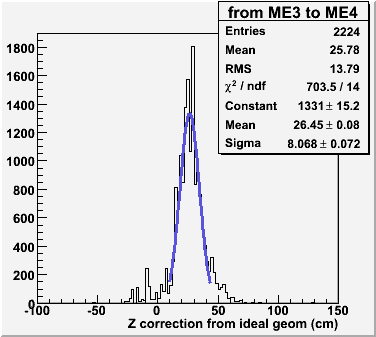
\includegraphics[width=0.4\linewidth]{hist_3and4.png}

\end{frame}

\begin{frame}
\frametitle{Consistency}
\small

\begin{itemize}
\item ME1
\begin{itemize}
\item 374.178~cm
\end{itemize}

\item ME2 ($\Delta$ = 8.6~cm)
\begin{itemize}
\item 391.11~cm
\item ME1 + 8.296~cm = 382.474~cm
\end{itemize}

\item ME3 ($\Delta$ = 5.7~cm, 3.2~cm, 8.9~cm)
\begin{itemize}
\item 388.00~cm
\item ME1 + 8.16~cm = 382.34~cm
\item ME2 + 0.1205~cm = 391.23~cm or 382.59~cm
\end{itemize}

\item ME4 ($\Delta$ = 12~cm, 0.43~cm, 9.9~cm, 12~cm, 2.2~cm, 10~cm)
\begin{itemize}
\item 424.34~cm
\item ME1 + 38.1~cm = 412.3~cm
\item ME2 + 33.66~cm = 424.77~cm
\item ME3 + 26.45~cm = 414.45~cm
\end{itemize}
\end{itemize}

\vfill About 10~cm consistency, but it really depends where the track
comes from (size of tracking volume, closeness to target, number of
tracks)

\end{frame}

\begin{frame}
\frametitle{ME2 and ME3 are linked?}

I haven't been able to verify this, but I'm pretty sure ME2 and ME3 are on opposite sides of the same yoke

\vfill All parameters agree to high precision (unlike other pairs)

\vfill Position of ME3 relative to ME2:

\begin{itemize}
\item $\Delta x$, $\Delta y$, $\Delta z$ = -0.26~mm, -0.36~mm, 1.52~mm
\item $\Delta \phi_x$, $\Delta \phi_y$, $\Delta \phi_z$ = 0.75~mrad, -0.78~mrad, 0.075~mrad
\end{itemize}

\end{frame}

\begin{frame}
\frametitle{Conclusions, what to do next}
\scriptsize

\begin{itemize}\setlength{\itemsep}{0.2 cm}
\item CSC Overlaps procedure either discovered a radial offset in
  ideal geometry or suffers from a problem due to wire granularity or
  both
\item Migrate CSC Overlaps procedure from local $x$ to raw strip
  measurements (6~mm RMS $\to$ 200~$\mu$m) in both track-fits and hit
  measurements; removes sensitivity to wires altogether
\item That will require a little infrastructure work
\item Baseline procedure can find stations using StandAloneMuon tracking
\item But it doesn't look like it will find radial positions with
  sufficient precision
\item I should apply Pablo's barrel alignment in this study, but wheel
  positions are key
\item I will, however, be able to align individual chambers in ME2 and
  ME3 due to the high statistics in the ME2 $\leftrightarrow$ ME3
  sample (not relative to barrel)
\item Statistics pointing to ME4 are poor: if comparison with hardware
  must be in ME4 (as we planned) we'll need to wait for improvements
  to CSC Overlaps procedure
\item CRUZET-3 tracker-to-muon alignment
\end{itemize}
\label{numpages}
\end{frame}

\end{document}
